%%%%%%%%%%%%%%%%%%%%%%%%%%
%                          %
% ----- INTRODUCTION ----- %
%                          %
%%%%%%%%%%%%%%%%%%%%%%%%%%

\section{Wordcloud}

	\subsection{Concept}

		Le wordcloud montre à l'utilisateur la liste des mots qu'il lit le plus fréquemment. Le visualisation est un amassage de mots de différentes tailles, placés d'une manière aléatoire sur un rectangle. Les mots les plus lus ont une taille plus grande afin d'attirer l'attention de l'utilisateur.

		Cette visualisation cherche à donner très rapidement une impression générale des thèmes que l'utilisateur parcourt lors de sa navigation.

		\begin{figure}[!h]
			\centering
			\subfloat[Maquette initiale de la vue]{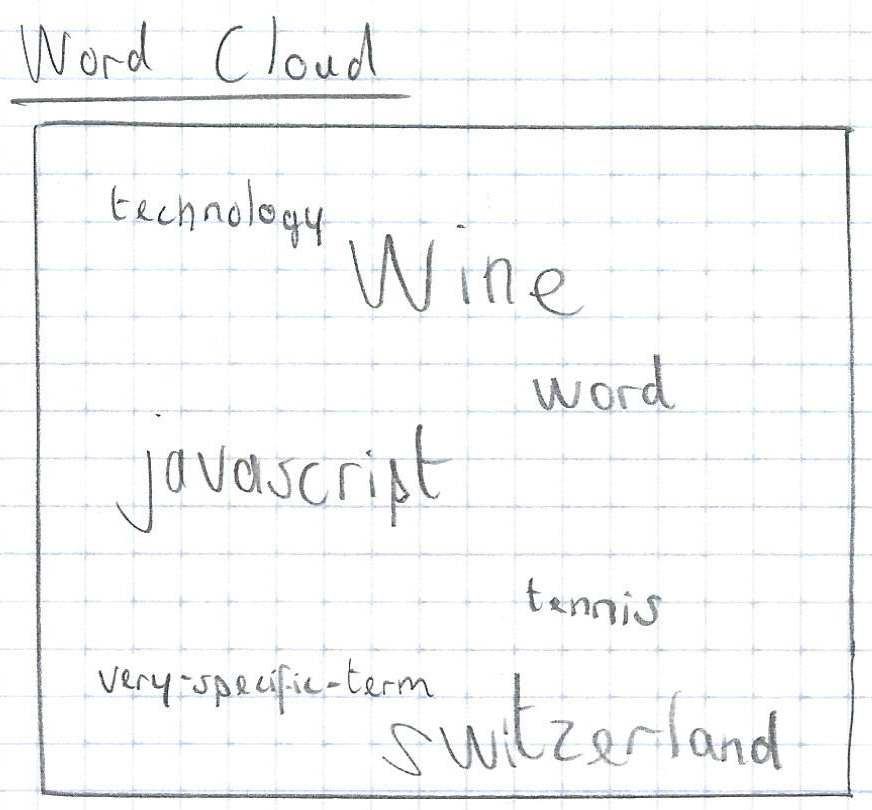
\includegraphics[width=0.3\textwidth,valign=t]{images/design/pages/wordcloud_mockup}}
			\subfloat[Exemple de résultat final]{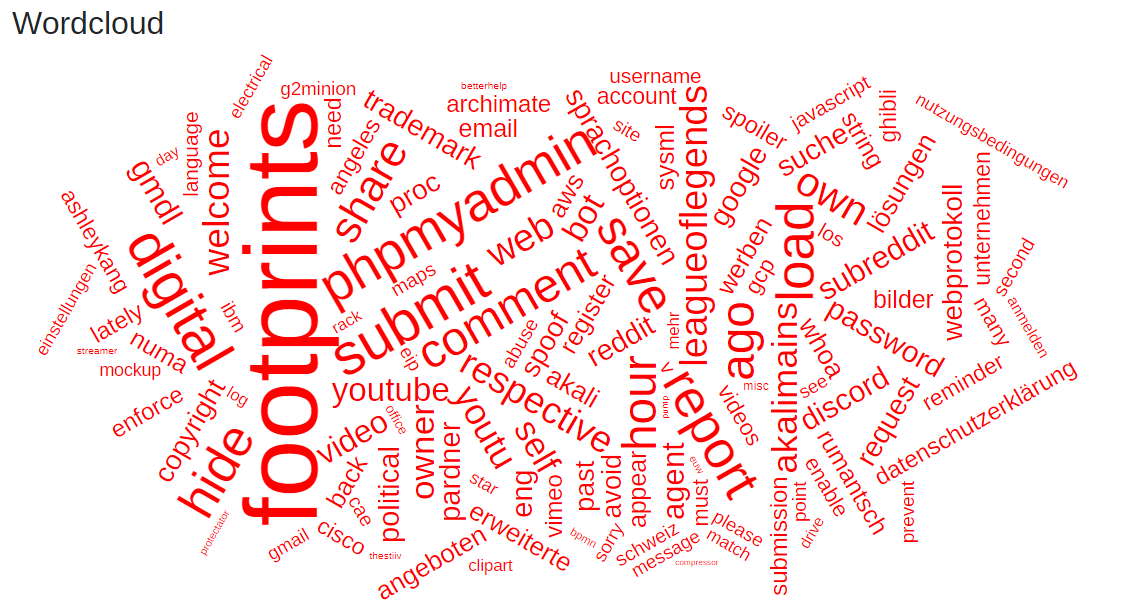
\includegraphics[width=0.6\textwidth,valign=t]{images/design/pages/wordcloud_final}}
			\caption{Maquette initiale et résultat final de la vue Wordcloud}
			\label{wordcloud_images}
		\end{figure}

		La figure~\ref{wordcloud_images} montre la différence entre la vue imaginée initialement et le résultat final.

	\subsection{Données}

		\subsubsection{Sources}

			Les données source servant à constituer cette visualisation sont :
			\begin{description}
				\item[Temps de visualisation] : Temps de visualisation total de chaque page 
				\item[Poids TF-IDF] : Poids final selon l'algorithme TF-IDF de chaque mot
			\end{description}

		\subsubsection{Algorithme}

			Afin de déterminer quels sont les mots affichés ainsi que leur taille sur la visualisation, on assigne un "poids" à chaque mot.

			La figure~\ref{wordcloud_algo} illustre le fonctionnement de l'algorithme utilisé :
			\begin{itemize}
				\item On effectue la somme du temps que l'utilisateur a passé à regarder chaque page visitée. Cette opération est effectuée sur le serveur, et l'interface obtient ce résultat en appelant l'endpoint \texttt{/api/mostWatchedSites} du serveur. Le résultat de cet appel est une liste de l'ensemble des pages web visitées, comprenant entre autres pour chaque page : 
				\begin{itemize}
					\item Son URL
					\item Le temps total de visite, en secondes
					\item Une liste des mots les plus significatifs selon TF-IDF ainsi que leur poids TF-IDF (normalisé entre 0 et 1)
				\end{itemize}
				\item On initialise un dictionnaire qui va contenir le poids de chaque mot.
				\item Pour chaque page web, on multiplie l'indice TF-IDF de chaque mot avec le temps de visualisation de la page. On additionne ce résultat au poids actuel du mot.
				\item Une fois tous les mots de toutes les pages web traités, nous sommes en possession d'un dictionnaire nous indiquant le poids final de chaque mot. Ce poids est donc égal à la somme de l'indice TF-IDF du mot sur chaque page multiplié par le temps de visite sur cette page.
				\item On trie les mots par leur poids final, et on ne conserve que les 200 premiers. Il s'agira des 200 mots présents sur le wordcloud.
				\item Pour chacun des 200 mots, leur taille sur le Wordcloud est égale à leur poids final.
			\end{itemize}

			\begin{figure}[!h]
				\centering
				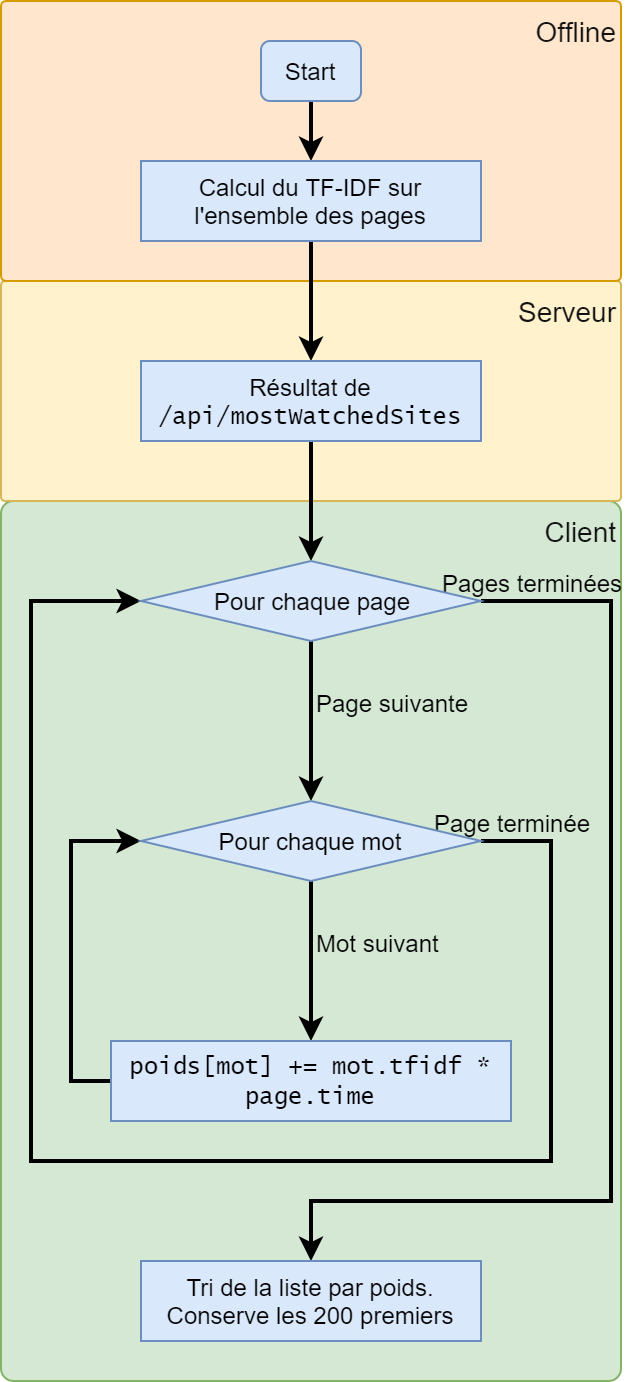
\includegraphics[height=1\textwidth]{images/design/pages/wordcloud_algo}
				\caption{Algorithme utilisé pour le Wordcloud}
				\label{wordcloud_algo}
			\end{figure}

	\subsection{Implémentation}

		\subsubsection{Serveur}

			La somme du temps de visualisation des pages est calculée en direct par une commande MySQL, elle est donc constamment à jour.

			Le poids TF-IDF de chaque mot est stocké dans la base de données, mais n'est pas constamment rafraîchi. L'opération de calcul des poids TF-IDF est une opération ponctuelle qui doit être lancée sur l'entièreté de la base de données par l'administrateur. Cette opération ne nécessite cependant pas de redémarrage du serveur.

			La concaténation de ces résultats (ainsi que certains autres qui ne sont pas utilisés par cette visualisation) est servie par l'endpoint \texttt{/api/mostWatchedSites} dans une liste en JSON.

		\subsubsection{Interface}

			La page va s'occuper d'agréger les résultats reçus du serveur. Ensuite, elle utilise les librairies \texttt{d3-cloud} ainsi que \texttt{d3} pour générer la visualisation du Wordcloud.

\newpage

\section{Topics List}

	\subsection{Concept}

		Le "Topics List" cherche à rassembler les mots en thèmes, et montre d'une manière plus synthétique les thèmes estimés que l'utilisateur parcourt fréquamment. À chaque thème est lié un ou plusieurs mots, qui reprèsentent le thème d'une manière générale. Chaque cercle du graphe représente soit un thème, soit un mot.

		Le but de cette visualisation est de montrer que nous pouvons déduire des thèmes et ainsi montrer un traitement plus fin des intérêts de l'utilisateur, que simplement additionner une liste de mots. Dans le marketing, les thèmes découverts pourraient être utilisés pour labelliser les utilisateurs à qui faire apparaître une publicité.

		\begin{figure}[!h]
			\centering
			\subfloat[Maquette initiale de la vue]{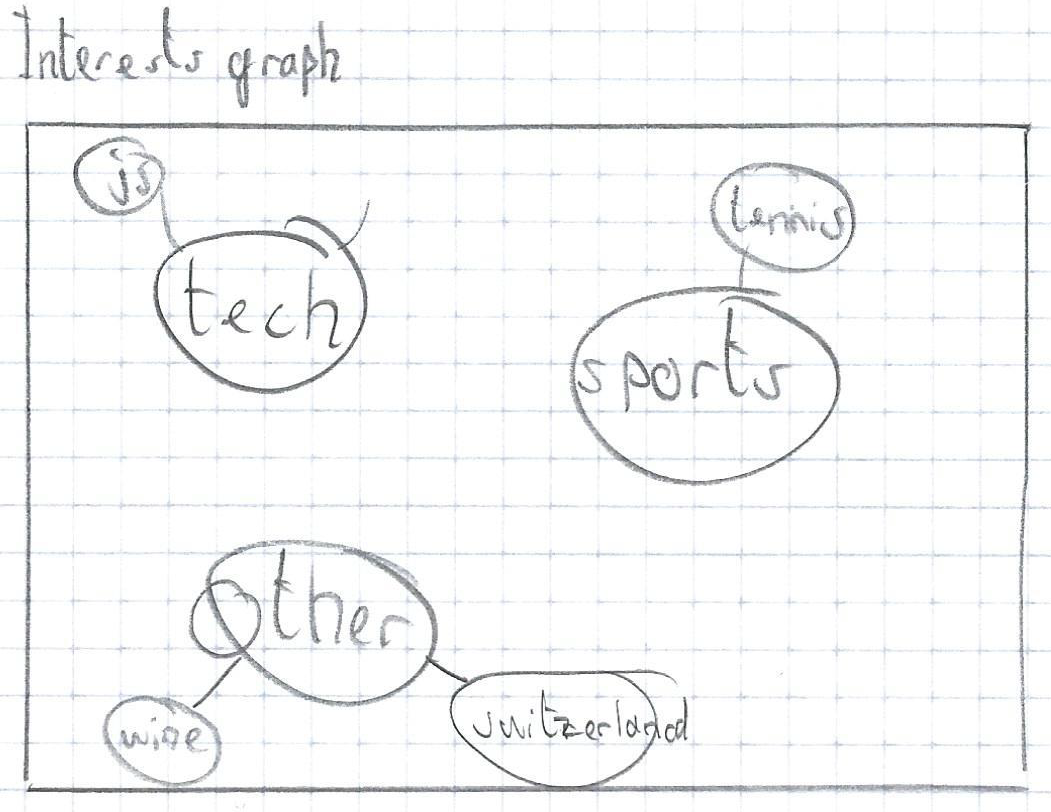
\includegraphics[width=0.32\textwidth,valign=t]{images/design/pages/topics_mockup}}
			\subfloat[Exemple de résultat final]{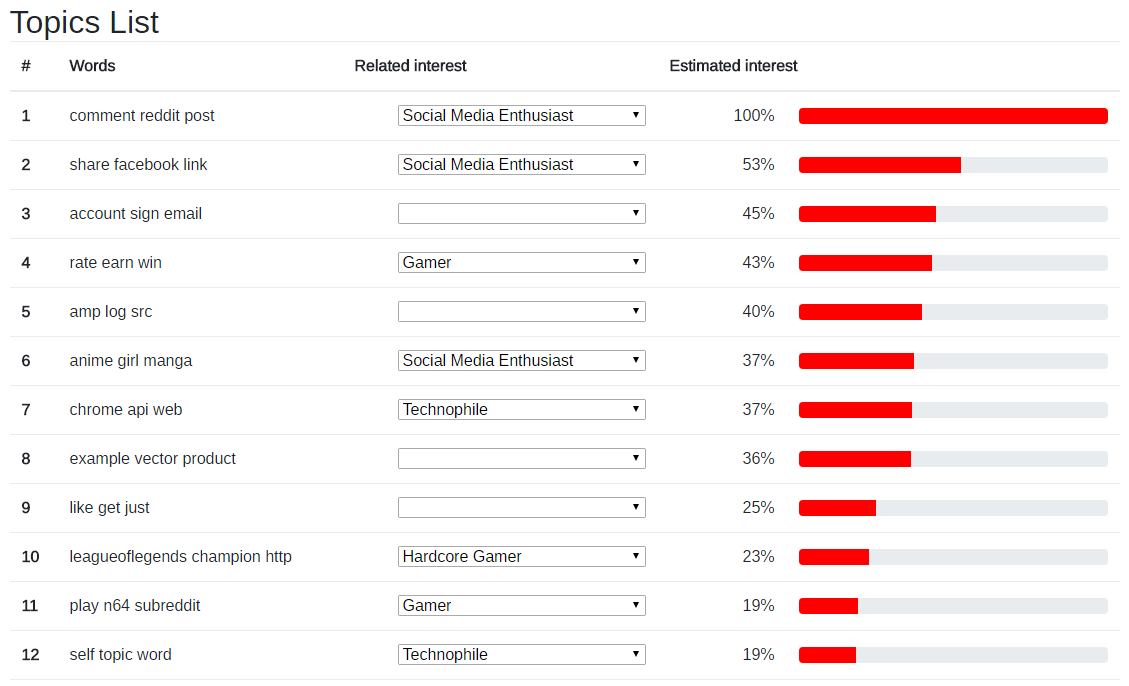
\includegraphics[width=0.62\textwidth,valign=t]{images/design/pages/topics_final}}
			\caption{Maquette initiale et résultat final de la vue Wordcloud}
			\label{topics_images}
		\end{figure}

		La figure~\ref{topics_images} montre la différence entre la vue imaginée et le résultat final. On note ici que le principe même de la vue ainsi que son nom sont différents qu'initialement.

	\subsection{Données}

		\subsubsection{Sources}

			Les données source servant à constituer cette visualisation sont :
			\begin{description}
				\item[Temps de visualisation] : Temps de visualisation total de chaque page 
				\item[Topics LDA] : Liste des topics générés par le modèle LDA
				\item[Topics par page] : Liste pré-caluclée des topics trouvés pour chaque page
				\item[Intérêts utilisateur] : Liste des intérêts renseignés par l'utilisateur
				\item[Correspondances topic-intrêt] : Liste des correspondances entre topic et intérêt renseignés par l'utilisateur 
			\end{description}

		\subsubsection{Algorithme}

			Afin de déterminer quels sont les topics affichés ainsi que leur intérêt estimé, on assigne un "score" à chaque topic pour l'utilisateur.

			L'algorithme suivant, illustré par la figure~\ref{topics_algo}, est appliqué aux données sources :
			\begin{itemize}
				\item On entraîne un modèle LDA avec un nombre défini de topics (typiquement 100) sur le contenu de l'ensemble des pages web,  une page web représentant un document.
				\item Une fois le modèle LDA entraîné, on lui demande la liste des 100 topics générés par leur représentation en 5 mots. Cette liste de topics est enregistrée dans la base de données.
				\item Pour chaque page enregistrée, on demande au modèle LDA quels sont les 5 topics les plus probables avec leur score de probabilité. Ces informations sont également enregistrées dans la base de données. Jusqu'ici, toutes ces opérations sont donc déjà calculées et se font avant le lancement du serveur. Elles ne sont pas mises à jour en temps réel.
				\item On effectue la somme du temps que l'utilisateur a passé à regarder chaque page visitée. Cette opération est effectuée sur le serveur, et l'interface obtient ce résultat en appelant l'endpoint \texttt{/api/mostWatchedSites} du serveur. Le résultat de cet appel est une liste de l'ensemble des pages web visitées, comprenant entre autres pour chaque page : 
				\begin{itemize}
					\item Son URL
					\item Le temps total de visite, en secondes
					\item Une liste des topics les plus significatifs selon le modèle LDA ainsi que leur probabilité
				\end{itemize}
				\item On initialise un dictionnaire qui va contenir le score de chaque topic.
				\item Pour chaque page web, on multiplie la probabilité de chaque topic LDA avec le temps de visualisation de la page. On additionne ce résultat au score actuel du topic.
				\item Une fois tous les topics de toutes les pages web traités, nous sommes en possession d'un dictionnaire nous indiquant le score final de chaque topics. Ce score est donc égal à la somme de la probabilité du topic sur chaque page multiplié par le temps de visite sur cette page.
				\item On trie les topics par leur score final, et on ne conserve que les 20 premiers. Il s'agira des 20 topics présents sur la page.
				\item On sélectionne les centres d'intérêt de l'utilisateur, ainsi que les associations qu'il a déjà crée pour le modèle LDA actuel. On ajoute les associations aux topics de l'interface.
			\end{itemize}

			\begin{figure}[!h]
				\centering
				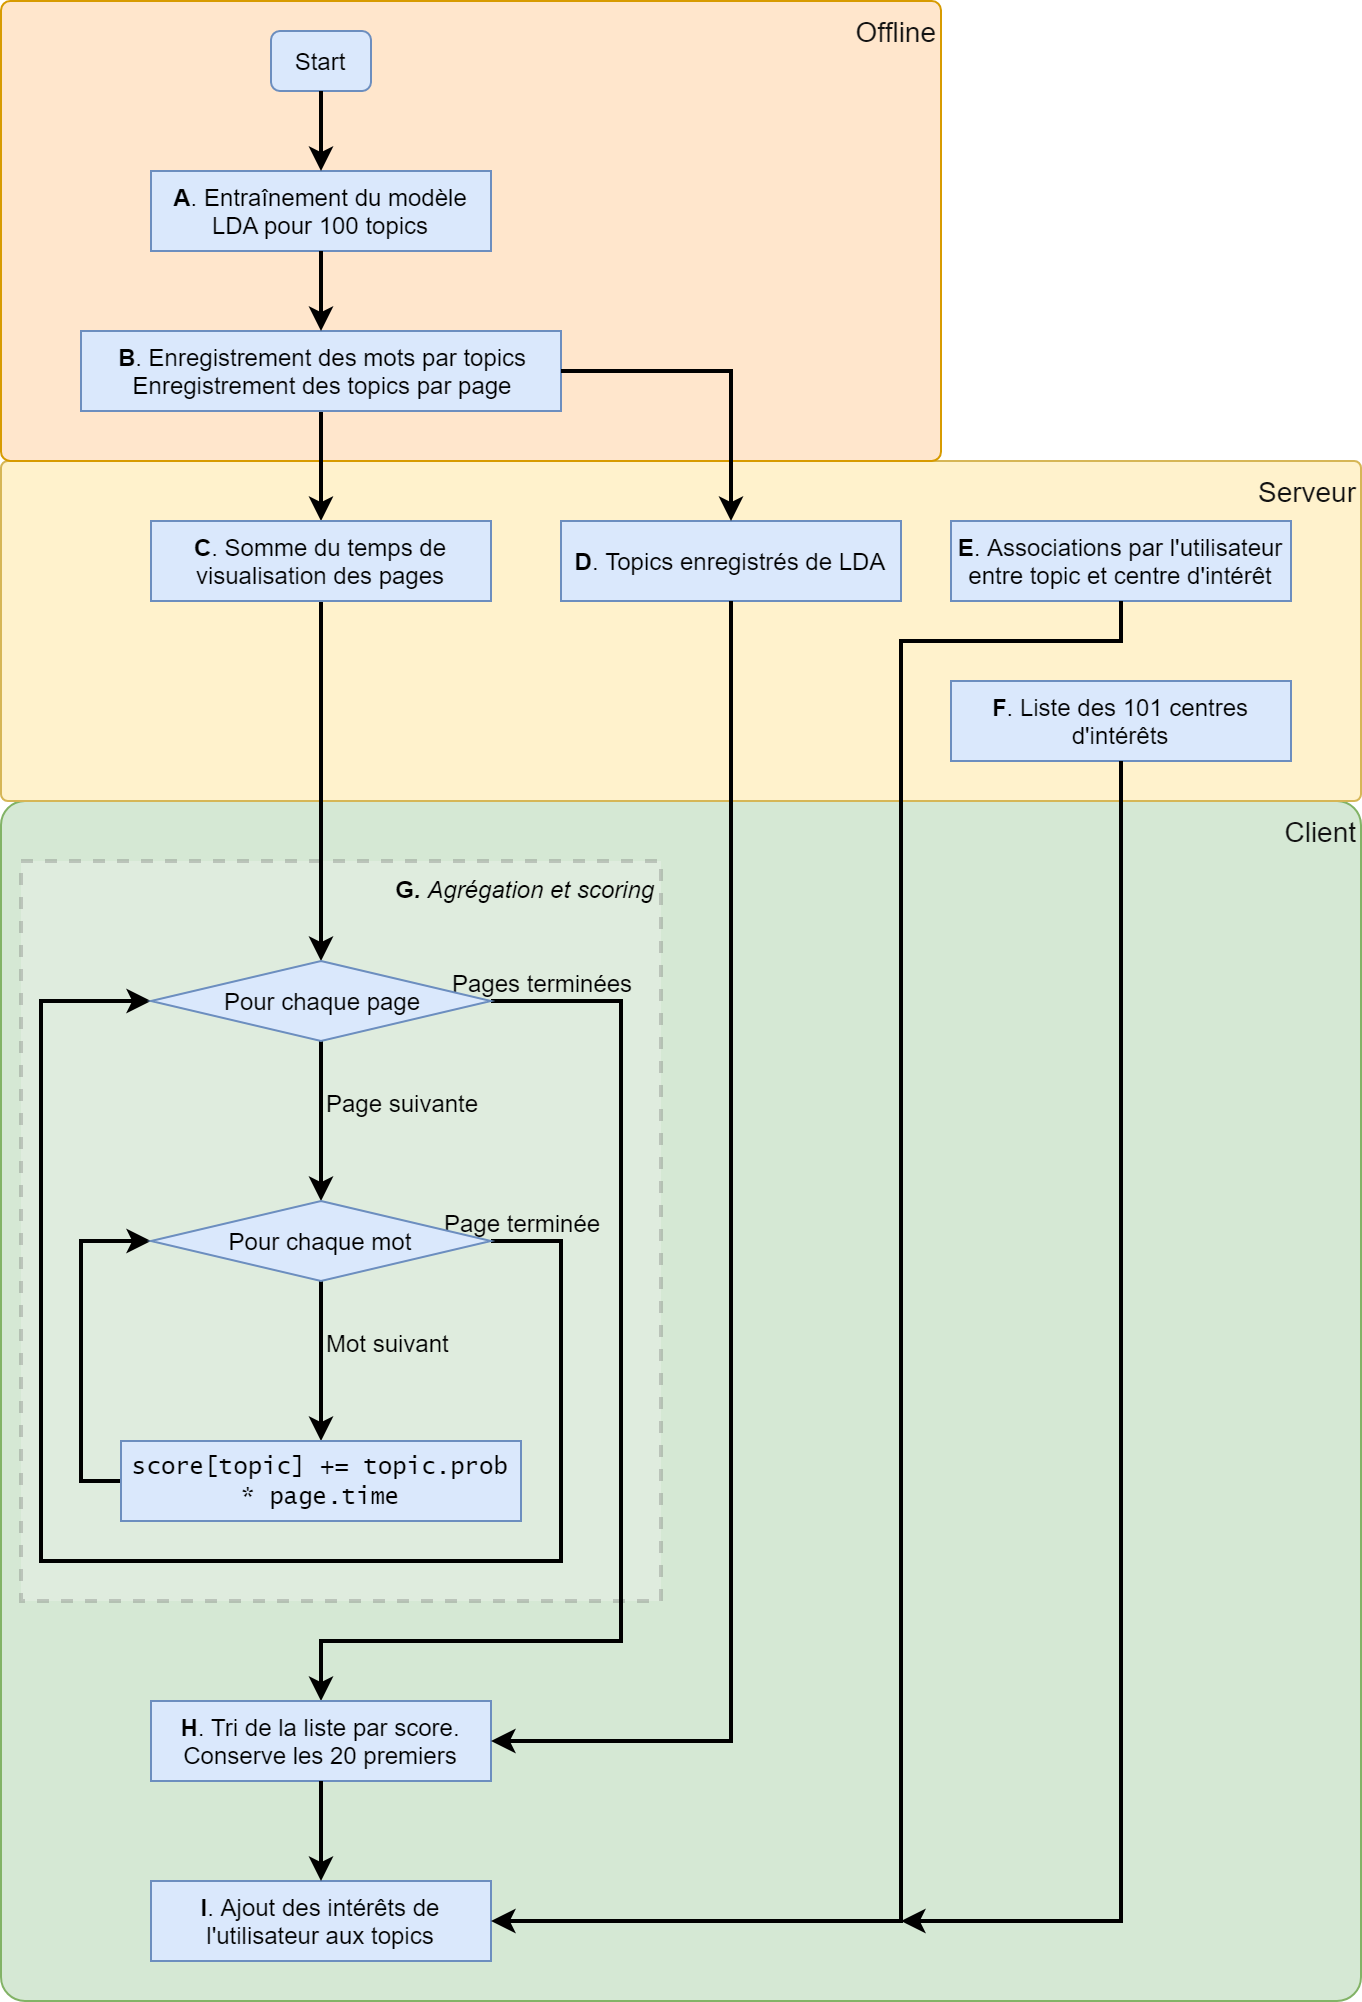
\includegraphics[height=1.3\textwidth]{images/design/pages/topics_algo}
				\caption{Algorithme utilisé pour le Topics List}
				\label{topics_algo}
			\end{figure}

	\subsection{Implémentation}

		\subsubsection{Serveur}

			La somme du temps de visualisation des pages est calculée en direct par une commande MySQL, elle est donc constamment à jour.

			Le modèle LDA est enregistré sur le disque local, et les résultats pré-calculés sont stocké dans la base de données, tout ceci n'est donc pas constamment rafraîchi. L'opération d'entraînement du modèle LDA est une opération ponctuelle qui doit être lancée sur l'entièreté de la base de données par l'administrateur. Cette opération nécessite le redémarrage du serveur, car de nombreuses mesures temporaires sont touchées.

			La concaténation de ces résultats (ainsi que certains autres qui ne sont pas utilisés par cette visualisation) est servie par l'endpoint \texttt{/api/mostWatchedSites} dans une liste en JSON. L'endpoint \texttt{/api/interestsList} est utilisé pour afficher le nom des centres d'intérêts, et l'endpoint \texttt{/api/getCurrentTags} donne l'ensemble des associations que l'utilisateur a crée entre ses centres d'intérêts, et les topics LDA actuels.

		\subsubsection{Interface}

			La page va s'occuper d'agréger les résultats reçus du serveur. La liste est ensuite générée sous forme d'un tableau HTML. Les barres d'intérêt sont des éléments \texttt{progressbar} venant de Bootstrap.

\section{Most Watched}

	\subsection{Concept}

	\subsection{Données}

		\subsubsection{Sources}

		\subsubsection{Algorithme}

	\subsection{Implémentation}

		\subsubsection{Client}

		\subsubsection{Interface}

\section{History}

	\subsection{Concept}

	\subsection{Données}

		\subsubsection{Sources}

		\subsubsection{Algorithme}

	\subsection{Implémentation}

		\subsubsection{Client}

		\subsubsection{Interface}